\section{Introduction}

\begin{figure}[t]
    \centering
    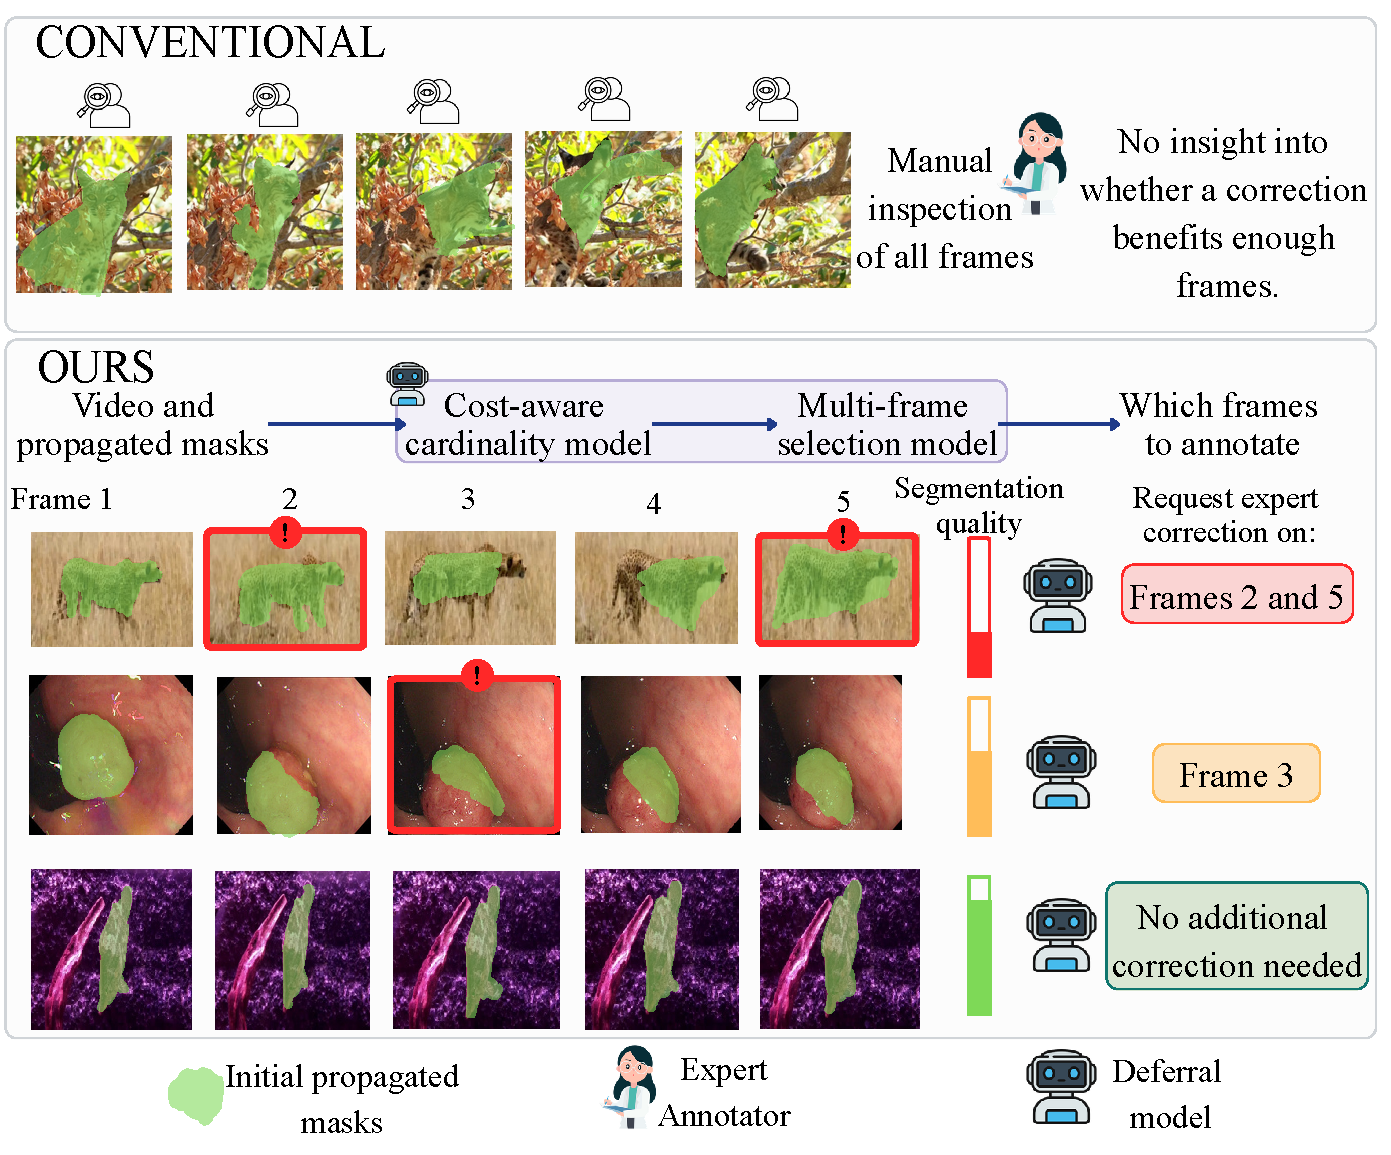
\includegraphics[width=\columnwidth]{Figures/Lteaser.pdf}
    \caption{
    Conventional correction requires an expert to inspect the propagated masks and decide where to intervene, without knowing whether a correction will improve only nearby frames or benefit the video more broadly. This can underuse expert effort by spending it on corrections with limited benefit. Our framework instead accounts for intervention cost and decides whether video correction is worthwhile, how many frames should be corrected, and where those corrections should be placed.
    }
    \label{fig:teaser}
\end{figure}

Recent promptable segmentation models such as SAM2~\cite{ravi2025sam} can segment objects throughout a video from a small number of mask, box, or point prompts.
Propagation from these prompts can nevertheless become inaccurate under appearance change, occlusion, rapid motion, and background similarity~\cite{hao2025interactive}.
Experts must then inspect the propagated segmentation and place corrective prompts~\cite{ozbulak2025revisiting}.
Each inspection and each corrective prompt incurs a cost, which makes corrective prompting a human--AI decision
problem: whether to request expert assistance, how many corrections are justified, and on which frames to place them.

Existing frame-selection approaches address where corrections should be placed, scoring candidate frames by uncertainty, predicted mask quality, expected improvement, or diversity~\cite{IVOSW,delatolas2024learning,vujasinovic2024strike}.
Each candidate is scored independently, so a set assembled from the highest-scoring frames can spend several corrections on the same failure while leaving others untouched.
These approaches also operate under a predefined annotation budget, fixing the number of corrections in advance rather than inferring it from the quality of the current propagation.
Approaches that avoid a fixed budget instead correct one frame at a time, alternating propagation, expert review, and annotation after every intervention \cite{vujasinovic2024strike}.

A related decision has been studied extensively in classification through learning to defer (L2D), which learns when expert intervention is warranted by explicitly balancing prediction quality against the cost of consulting an expert~\cite{verma2022calibrated,mozannar2020consistent}.
Conventional formulations choose between retaining a machine prediction and replacing it with an expert one, and recent extensions also learn how many experts to consult for each input~\cite{zhang2024learning,montreuil2025ask}.
L2RP~\cite{rasanjalee2026understanding} brings this reasoning to promptable video segmentation, deciding whether to retain the current propagation or request a correction on one selected frame.
However, L2RP can request
at most one correction for the entire video, which may be insufficient
when propagation errors occur in multiple parts of the video.
In each case, the consultations are treated as independent, but a corrective prompt re-propagates through the video, so the number of corrections worth requesting depends on which frames receive them.

We therefore formulate corrective prompting as a
\textit{variable-cardinality learning-to-defer} problem.
Given the current propagated segmentation and a specified expert cost,
our framework determines whether expert assistance is needed, how many
corrective prompts to request, and which frames should receive them.
The selected frames are constructed as a complementary set rather than
ranked independently, allowing each choice to account for the frames
already selected. All corrections are then requested in a single batch
and incorporated through one re-propagation, avoiding the repeated
expert-interaction and propagation rounds required by sequential
correction methods.

Our main contributions are as follows:
\begin{itemize}
    \item We formulate corrective prompting for promptable video
    segmentation as a variable-cardinality learning-to-defer problem,
    where the system jointly determines whether correction is needed,
    how many frames should be corrected, and which frames should be
    selected.

    \item We propose a framework that combines a cardinality model for
    determining how many corrections are warranted under a given expert cost
    with a multi-frame selection model for selecting the corresponding frames,
    with all expert prompts requested in a single correction round.

    \item We evaluate our framework on four datasets spanning object
    transformation, camouflage, colonoscopy, and thyroid ultrasound,
    comparing it against fixed-budget frame-selection methods and adapted
    learning-to-defer baselines.
\end{itemize}
